\documentclass[hyperref, a4paper]{article}

\usepackage{geometry}
\usepackage{titling}
\usepackage{titlesec}
% No longer needed, since we will use enumitem package
% \usepackage{paralist}
\usepackage{enumitem}
\usepackage{footnote}
\usepackage{enumerate}
\usepackage{amsmath, amssymb, amsthm}
\usepackage{mathtools}
\usepackage{bbm}
\usepackage{graphicx}
\usepackage{subcaption}
\usepackage{physics}
\usepackage{tensor}
\usepackage{siunitx}
\usepackage[version=4]{mhchem}
\usepackage{tikz}
\usepackage{xcolor}
\usepackage{listings}
\usepackage{autobreak}
\usepackage[ruled, vlined, linesnumbered]{algorithm2e}
\usepackage{nameref,zref-xr}
\zxrsetup{toltxlabel}
\usepackage[sorting=none]{biblatex}
\addbibresource{theory.bib}
\addbibresource{experiments.bib}
\usepackage[colorlinks,unicode]{hyperref} % , linkcolor=black, anchorcolor=black, citecolor=black, urlcolor=black, filecolor=black
\usepackage[most]{tcolorbox}
\usepackage{prettyref}

% Page style
\geometry{left=3.18cm,right=3.18cm,top=2.54cm,bottom=2.54cm}
\titlespacing{\paragraph}{0pt}{1pt}{10pt}[20pt]
\setlength{\droptitle}{-5em}

% More compact lists 
\setlist[itemize]{
    itemindent=17pt, 
    leftmargin=1pt,
    listparindent=\parindent,
    parsep=0pt,
}

% Math operators
\DeclareMathOperator{\timeorder}{\mathcal{T}}
\DeclareMathOperator{\diag}{diag}
\DeclareMathOperator{\legpoly}{P}
\DeclareMathOperator{\primevalue}{P}
\DeclareMathOperator{\sgn}{sgn}
\DeclareMathOperator{\res}{Res}
\newcommand*{\ii}{\mathrm{i}}
\newcommand*{\ee}{\mathrm{e}}
\newcommand*{\const}{\mathrm{const}}
\newcommand*{\suchthat}{\quad \text{s.t.} \quad}
\newcommand*{\argmin}{\arg\min}
\newcommand*{\argmax}{\arg\max}
\newcommand*{\normalorder}[1]{: #1 :}
\newcommand*{\pair}[1]{\langle #1 \rangle}
\newcommand*{\fd}[1]{\mathcal{D} #1}
\DeclareMathOperator{\bigO}{\mathcal{O}}

% TikZ setting
\usetikzlibrary{arrows,shapes,positioning}
\usetikzlibrary{arrows.meta}
\usetikzlibrary{decorations.markings}
\tikzstyle arrowstyle=[scale=1]
\tikzstyle directed=[postaction={decorate,decoration={markings,
    mark=at position .5 with {\arrow[arrowstyle]{stealth}}}}]
\tikzstyle ray=[directed, thick]
\tikzstyle dot=[anchor=base,fill,circle,inner sep=1pt]

% Algorithm setting
% Julia-style code
\SetKwIF{If}{ElseIf}{Else}{if}{}{elseif}{else}{end}
\SetKwFor{For}{for}{}{end}
\SetKwFor{While}{while}{}{end}
\SetKwProg{Function}{function}{}{end}
\SetArgSty{textnormal}

\newcommand*{\concept}[1]{{\textbf{#1}}}

% Embedded codes
\lstset{basicstyle=\ttfamily,
  showstringspaces=false,
  commentstyle=\color{gray},
  keywordstyle=\color{blue}
}

% Reference formatting
\newrefformat{fig}{Fig.~\ref{#1}}
\newcommand*{\term}[1]{\textit{#1}}

% Color boxes
\tcbuselibrary{skins, breakable, theorems}

\newtcbtheorem{infobox}{Box}{
    enhanced,
    boxrule=0pt,
    colback=blue!5,
    colframe=blue!5,
    coltitle=blue!50,
    borderline west={4pt}{0pt}{blue!65},
    sharp corners,
    fonttitle=\bfseries, 
    breakable,
    before upper={\parindent15pt\noindent}}{box}
\newtcbtheorem[use counter from=infobox]{theorybox}{Box}{
    enhanced,
    boxrule=0pt,
    colback=orange!5, 
    colframe=orange!5, 
    coltitle=orange!50,
    borderline west={4pt}{0pt}{orange!65},
    sharp corners,
    fonttitle=\bfseries, 
    breakable,
    before upper={\parindent15pt\noindent}}{box}
\newtcbtheorem[use counter from=infobox]{learnbox}{Box}{
    enhanced,
    boxrule=0pt,
    colback=green!5,
    colframe=green!5,
    coltitle=green!50,
    borderline west={4pt}{0pt}{green!65},
    sharp corners,
    fonttitle=\bfseries, 
    breakable,
    before upper={\parindent15pt\noindent}}{box}


\newenvironment{shelldisplay}{\begin{lstlisting}}{\end{lstlisting}}

\newcommand*{\kB}{k_{\text{B}}}
\newcommand*{\muB}{\mu_{\text{B}}}
\newcommand*{\efermi}{E_{\text{F}}}
\newcommand*{\pfermi}{p_{\text{F}}}
\newcommand*{\vfermi}{v_{\text{F}}}
\newcommand*{\sA}{\text{A}}
\newcommand*{\sB}{\text{B}}
\newcommand*{\Tc}{T_{\text{c}}}
\newcommand*{\hethree}{$^3$He}
\newcommand*{\hefour}{$^4$He}

\title{Fermi liquid}
\author{Jinyuan Wu}

\begin{document}

\maketitle

\section{Free electron gas}

A free electron gas is described by%
\footnote{
    For some reason, 
    when talking about Fermi liquid, 
    people like to use $\vb*{p}$ instead of $\vb*{k}$.
}
\begin{equation}
    H = \sum_i \frac{\vb*{p}_i^2}{2m},
\end{equation}
and we get a Fermi sphere in the momentum space 
containing all occupied states, 
and a Fermi momentum $\pfermi$.
After we add a periodic potential $V(\vb*{r})$ to the model, 
we get \concept{bands}: 
parabolic bands are displaced periodically 
according to the $\vb*{G}$-grid, 
and the crossing points of these curves 
undergo degeneracy breaking,
and the spectrum, eventually, 
becomes several bands confined in the first Brillouin zone. 
Despite this correction, 
the number of filled electrons never changes.

For a free electron gas, we have well-known observables like 
the density of states at $\efermi$ 
(here $\omega = \varepsilon - \efermi$)
\begin{equation}
    N(\omega = 0) = \frac{m}{\pi^2} \frac{\pfermi}{\hbar^3}, 
    \label{eq:free-electron.dos}
\end{equation}
the electronic specific heat 
\begin{equation}
    C_v = \underbrace{\frac{\pi^2 \kB^2}{3} N(\omega = 0)}_{\text{Sommerfield $\gamma$}} \cdot \ T, 
    \label{eq:free-electron.specific-heat}
\end{equation}
and the magnetic susceptibility 
\begin{equation}
    \chi = \mu_0  \muB^2 \cdot N(\omega = 0).
\end{equation}

\hethree{} atoms are fermions: 
we have two electrons, two protons, and only one neutron
in one \hethree{} atom, 
and therefore there are odd fermions inside 
and the composite state is a fermion. 
In a \hethree{} liquid, 
since the distance between the atoms is drastically reduced, 
we can expect the effect of repulsion is much stronger 
than the case in the gas phase. 
This is a cold atom model of electrons in solids: 
we can easily measure the specific heat, etc. 
of the liquid \hethree.

\begin{figure}
    \centering
    \begin{tikzpicture}[x=0.75pt,y=0.75pt,yscale=-0.75,xscale=0.75]
    %uncomment if require: \path (0,300); %set diagram left start at 0, and has height of 300
    
    %Straight Lines [id:da6815322853947638] 
    \draw    (108,249) -- (359.83,249) ;
    \draw [shift={(361.83,249)}, rotate = 180] [fill={rgb, 255:red, 0; green, 0; blue, 0 }  ][line width=0.08]  [draw opacity=0] (12,-3) -- (0,0) -- (12,3) -- cycle    ;
    %Straight Lines [id:da7841735564914218] 
    \draw    (108,249) -- (108,55.52) ;
    \draw [shift={(108,53.52)}, rotate = 90] [fill={rgb, 255:red, 0; green, 0; blue, 0 }  ][line width=0.08]  [draw opacity=0] (12,-3) -- (0,0) -- (12,3) -- cycle    ;
    %Curve Lines [id:da18279729625571206] 
    \draw    (108,249) .. controls (187.83,143.52) and (196.83,174.52) .. (243.83,167.52) .. controls (290.83,160.52) and (308.83,133.52) .. (329.83,109.52) ;
    %Straight Lines [id:da8082462725197179] 
    \draw  [dash pattern={on 4.5pt off 4.5pt}]  (108,249) -- (248.83,68.52) ;
    
    % Text Node
    \draw (108,50.52) node [anchor=south] [inner sep=0.75pt]    {$C_{V}$};
    % Text Node
    \draw (363.83,249) node [anchor=west] [inner sep=0.75pt]    {$T$};
    
    
    \end{tikzpicture}
    
    \caption{Heat capacity curve of liquid \hethree}
    \label{fig:he-heat-capacity}
\end{figure}

The $C_V$-$T$ curve measured looks like \prettyref{fig:he-heat-capacity}.
As is expected, 
when $T \to 0$, 
we see a $C_V \propto T$ behavior, 
qualitatively agreeing with \eqref{eq:free-electron.specific-heat}.
The coefficient however is not what is predicted by 
\eqref{eq:free-electron.dos} and
\eqref{eq:free-electron.specific-heat}.
Now if we apply pressure to liquid \hethree, 
$C_v / T$ clearly increases. 

For a fermion gas, 
we can measure the mass according to \eqref{eq:free-electron.specific-heat}
and \eqref{eq:free-electron.dos}. 
Now if we calculate the ``mass'' of \hethree according to the two equations, 
we get a pressure-dependent 
(quite surprising because the density of liquids almost stays the same when we press it)
``effective mass''
that is never the same as the bare mass of \hethree.

The next question, then, 
is whether liquid \hethree -- 
a system with known strong interaction -- 
can be equivalently described 
by something with the effective mass. 

\section{Assumptions of Fermi liquid theory}

\subsection{Motivation: what happens after interaction is turned on}\label{sec:collision-scaling}

The general form of Hamiltonian of fermionic systems 
that is found in condensed matter physics looks like 
\begin{equation}
    H = \sum_i \frac{\vb*{p}_i^2}{2m} + 
    \sum_{i, j} V(\abs{\vb*{r}_i - \vb*{r}_j}).
\end{equation}
When we deal with a two-body problem with this dynamics, 
the collision behavior is completely described
by the scattering cross-section. 
If we extend this picture to a many-body system,
we immediately see scattering changes 
the momentum distribution of particles, 
because the final states of scattering 
can obviously be over the Fermi surface, 
and therefore there is still some distribution above $\pfermi$ now
(\prettyref{fig:fermi-liquid-distribution}). 

\begin{figure}
    \centering
    \begin{tikzpicture}[x=0.75pt,y=0.75pt,yscale=-0.8,xscale=0.8]
    %uncomment if require: \path (0,300); %set diagram left start at 0, and has height of 300
    
    %Straight Lines [id:da009219527738367317] 
    \draw    (405,225) -- (617,225) ;
    \draw [shift={(619,225)}, rotate = 180] [fill={rgb, 255:red, 0; green, 0; blue, 0 }  ][line width=0.08]  [draw opacity=0] (12,-3) -- (0,0) -- (12,3) -- cycle    ;
    %Straight Lines [id:da2079961540240256] 
    \draw    (405,225) -- (405,84.5) ;
    \draw [shift={(405,82.5)}, rotate = 90] [fill={rgb, 255:red, 0; green, 0; blue, 0 }  ][line width=0.08]  [draw opacity=0] (12,-3) -- (0,0) -- (12,3) -- cycle    ;
    %Straight Lines [id:da25299815998590813] 
    \draw  [dash pattern={on 4.5pt off 4.5pt}]  (405,145.5) -- (512,145.5) ;
    %Straight Lines [id:da23611716817469208] 
    \draw  [dash pattern={on 4.5pt off 4.5pt}]  (512,145.5) -- (512,224.5) ;
    %Curve Lines [id:da9173257888464759] 
    \draw    (405,145.5) .. controls (500,143.5) and (519,226.5) .. (587,225) ;
    %Curve Lines [id:da006174472132643993] 
    \draw [draw opacity=0][fill={rgb, 255:red, 74; green, 144; blue, 226 }  ,fill opacity=0.5 ]   (405,146) .. controls (500,144) and (519,227) .. (587,225.5) .. controls (404,224) and (589,225) .. (405,225) .. controls (404,147) and (404,223) .. (405,146) -- cycle ;
    %Straight Lines [id:da4367238433084937] 
    \draw    (68,225) -- (280,225) ;
    \draw [shift={(282,225)}, rotate = 180] [fill={rgb, 255:red, 0; green, 0; blue, 0 }  ][line width=0.08]  [draw opacity=0] (12,-3) -- (0,0) -- (12,3) -- cycle    ;
    %Straight Lines [id:da3594146199392185] 
    \draw    (68,225) -- (68,84.5) ;
    \draw [shift={(68,82.5)}, rotate = 90] [fill={rgb, 255:red, 0; green, 0; blue, 0 }  ][line width=0.08]  [draw opacity=0] (12,-3) -- (0,0) -- (12,3) -- cycle    ;
    %Straight Lines [id:da3068774329734081] 
    \draw  [dash pattern={on 4.5pt off 4.5pt}]  (68,145.5) -- (175,145.5) ;
    %Straight Lines [id:da14782967759901622] 
    \draw  [dash pattern={on 4.5pt off 4.5pt}]  (175,145.5) -- (175,224.5) ;
    %Curve Lines [id:da7552878456427861] 
    \draw    (68,145.5) .. controls (110,144.5) and (137,146.5) .. (175,155.5) ;
    %Curve Lines [id:da40499842494527183] 
    \draw    (175,219.5) .. controls (195,222.5) and (217,224.5) .. (282,225) ;
    %Straight Lines [id:da31095032234024567] 
    \draw    (175,155.5) -- (175,219.5) ;
    %Curve Lines [id:da9323659415170968] 
    \draw [draw opacity=0][fill={rgb, 255:red, 74; green, 144; blue, 226 }  ,fill opacity=0.5 ]   (68,145.5) .. controls (131,145.5) and (120,144.5) .. (175,155.5) .. controls (176,220.5) and (174,159.5) .. (175,219.5) .. controls (227,224.5) and (229,225.5) .. (282,225) .. controls (83,223.5) and (262,226.5) .. (68,225) .. controls (69,151.5) and (67,226.5) .. (68,145.5) -- cycle ;
    %Straight Lines [id:da2726570766053802] 
    \draw [color={rgb, 255:red, 155; green, 155; blue, 155 }  ,draw opacity=1 ]   (175,155.5) -- (190,155.5) ;
    %Straight Lines [id:da794346269199613] 
    \draw [color={rgb, 255:red, 155; green, 155; blue, 155 }  ,draw opacity=1 ]   (175,219.5) -- (190,219.5) ;
    %Straight Lines [id:da8221957579922665] 
    \draw [color={rgb, 255:red, 155; green, 155; blue, 155 }  ,draw opacity=1 ]   (187,157.5) -- (187,217.5) ;
    \draw [shift={(187,219.5)}, rotate = 270] [fill={rgb, 255:red, 155; green, 155; blue, 155 }  ,fill opacity=1 ][line width=0.08]  [draw opacity=0] (12,-3) -- (0,0) -- (12,3) -- cycle    ;
    \draw [shift={(187,155.5)}, rotate = 90] [fill={rgb, 255:red, 155; green, 155; blue, 155 }  ,fill opacity=1 ][line width=0.08]  [draw opacity=0] (12,-3) -- (0,0) -- (12,3) -- cycle    ;
    
    % Text Node
    \draw (621,225) node [anchor=west] [inner sep=0.75pt]    {$k$};
    % Text Node
    \draw (405,79.5) node [anchor=south] [inner sep=0.75pt]    {$n_{k}$};
    % Text Node
    \draw (284,225) node [anchor=west] [inner sep=0.75pt]    {$k$};
    % Text Node
    \draw (68,79.5) node [anchor=south] [inner sep=0.75pt]    {$n_{k}$};
    % Text Node
    \draw (192,178) node [anchor=north west][inner sep=0.75pt]    {$Z$};
    % Text Node
    \draw (166,250) node [anchor=north west][inner sep=0.75pt]   [align=left] {(a)};
    % Text Node
    \draw (499,250) node [anchor=north west][inner sep=0.75pt]   [align=left] {(b)};
    
    
\end{tikzpicture}
    
    \caption{Two types of interaction correction to the electron distribution.
    (a) The Fermi liquid case: there is still a stepwise change of $n$ with respect to the energy.
    (b) The non-Fermi liquid case: the change of $n$ is smooth.}
    \label{fig:fermi-liquid-distribution}
\end{figure}

It should be noted that \prettyref{fig:fermi-liquid-distribution} 
is the distribution function concerning the momentum, not the energy:
we still have a very clear energy upper bound 
in the energy distribution function.
The reason of electron distribution over $\pfermi$
comes from the fact that $n(\vb*{p})$ is no longer a good quantum number 
after the interaction is turned on
and scattering occurs.
The electrons with $\abs*{\vb*{p}} > \pfermi$ 
still have energies \emph{below} the corrected Fermi energy
(\prettyref{fig:arpes-scheme}).
Sometimes people say that because scattering changes $\vb*{p}$, 
the momentum is no longer a good quantum number; 
what we want to point out here 
is it may also be possible 
that the single-electron picture completely breaks down 
(and we can't even talk about the momentum of a single electron).
If the interaction is strong enough, 
we may find $Z = 0$, 
and in the spectrum of the system we no longer have 
well-defined electron-like quasiparticles:
when an electron is injected into the system, 
it quickly excites many electron-hole pairs 
because of scattering
and decays.

\begin{figure}
    \centering
    \begin{tikzpicture}[x=0.75pt,y=0.75pt,yscale=-0.7,xscale=0.7]
    %uncomment if require: \path (0,523); %set diagram left start at 0, and has height of 523
    
    %Shape: Rectangle [id:dp7131803617577668] 
    \draw  [draw opacity=0][fill={rgb, 255:red, 74; green, 144; blue, 226 }  ,fill opacity=0.1 ] (196,288) -- (223.83,288) -- (223.83,473.85) -- (196,473.85) -- cycle ;
    %Straight Lines [id:da7598722594677334] 
    \draw    (266,474) -- (486.83,474) ;
    \draw [shift={(488.83,474)}, rotate = 180] [fill={rgb, 255:red, 0; green, 0; blue, 0 }  ][line width=0.08]  [draw opacity=0] (12,-3) -- (0,0) -- (12,3) -- cycle    ;
    %Image [id:dp8241642666901281] 
    \draw (360.92,369.08) node  {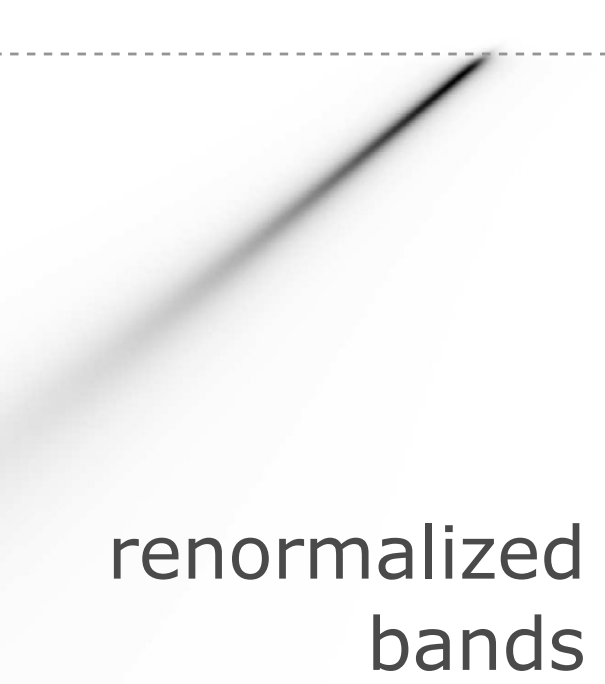
\includegraphics[width=100.71pt,height=100.71pt]{plot/arpes-spectrum-example-1.PNG}};
    %Straight Lines [id:da6586111996921291] 
    \draw    (266,474) -- (266,247.85) ;
    \draw [shift={(266,245.85)}, rotate = 90] [fill={rgb, 255:red, 0; green, 0; blue, 0 }  ][line width=0.08]  [draw opacity=0] (12,-3) -- (0,0) -- (12,3) -- cycle    ;
    %Straight Lines [id:da35625894168032457] 
    \draw    (224,474) -- (224,247.85) ;
    \draw [shift={(224,245.85)}, rotate = 90] [fill={rgb, 255:red, 0; green, 0; blue, 0 }  ][line width=0.08]  [draw opacity=0] (12,-3) -- (0,0) -- (12,3) -- cycle    ;
    %Straight Lines [id:da943265616635429] 
    \draw [color={rgb, 255:red, 74; green, 144; blue, 226 }  ,draw opacity=1 ]   (196,288) -- (223.83,288) ;
    %Straight Lines [id:da6139331520486002] 
    \draw [color={rgb, 255:red, 74; green, 144; blue, 226 }  ,draw opacity=1 ]   (196,288) -- (196.17,474) ;
    %Straight Lines [id:da8048536335889904] 
    \draw [color={rgb, 255:red, 74; green, 144; blue, 226 }  ,draw opacity=1 ]   (223.83,257.85) -- (223.83,288) ;
    %Straight Lines [id:da1675470318517831] 
    \draw  [dash pattern={on 0.84pt off 2.51pt}]  (223.83,288) -- (265.83,288) ;
    %Straight Lines [id:da12246512878622995] 
    \draw  [dash pattern={on 0.84pt off 2.51pt}]  (459.83,288) -- (501.83,288) ;
    %Straight Lines [id:da8543910261314052] 
    \draw    (223.83,473.85) -- (156.67,473.85) ;
    \draw [shift={(154.67,473.85)}, rotate = 360] [fill={rgb, 255:red, 0; green, 0; blue, 0 }  ][line width=0.08]  [draw opacity=0] (12,-3) -- (0,0) -- (12,3) -- cycle    ;
    %Straight Lines [id:da9955938989460331] 
    \draw    (266,195.85) -- (486.83,195.85) ;
    \draw [shift={(488.83,195.85)}, rotate = 180] [fill={rgb, 255:red, 0; green, 0; blue, 0 }  ][line width=0.08]  [draw opacity=0] (12,-3) -- (0,0) -- (12,3) -- cycle    ;
    %Straight Lines [id:da18702951363365972] 
    \draw    (266,195.85) -- (266,125.92) ;
    \draw [shift={(266,123.92)}, rotate = 90] [fill={rgb, 255:red, 0; green, 0; blue, 0 }  ][line width=0.08]  [draw opacity=0] (12,-3) -- (0,0) -- (12,3) -- cycle    ;
    %Straight Lines [id:da2056417168381537] 
    \draw  [dash pattern={on 0.84pt off 2.51pt}]  (419,125.31) -- (419,473.52) ;
    %Shape: Polygon Curved [id:ds2789435512931895] 
    \draw  [color={rgb, 255:red, 74; green, 144; blue, 226 }  ,draw opacity=1 ][fill={rgb, 255:red, 74; green, 144; blue, 226 }  ,fill opacity=0.1 ] (265.85,155.02) .. controls (332.6,156.3) and (406.6,152.55) .. (418.6,162.05) .. controls (419.13,175.27) and (418.38,162.27) .. (419.13,188.77) .. controls (429.13,194.02) and (434.13,194.77) .. (453.13,195.77) .. controls (406.13,195.77) and (360.38,195.77) .. (266,195.85) .. controls (266.1,155.52) and (266.35,195.77) .. (265.85,155.02) -- cycle ;
    %Straight Lines [id:da08475461712586241] 
    \draw  [dash pattern={on 0.84pt off 2.51pt}]  (265.85,155.02) -- (419.88,155.02) ;
    
    % Text Node
    \draw (490.83,474) node [anchor=west] [inner sep=0.75pt]    {$k$};
    % Text Node
    \draw (266,242.85) node [anchor=south] [inner sep=0.75pt]    {$\omega $};
    % Text Node
    \draw (224.19,242.85) node [anchor=south] [inner sep=0.75pt]  [rotate=-358.35]  {$\omega $};
    % Text Node
    \draw (503.83,288) node [anchor=west] [inner sep=0.75pt]    {$\varepsilon _{\text{F}}$};
    % Text Node
    \draw (152.67,473.85) node [anchor=east] [inner sep=0.75pt]   [align=left] {$\displaystyle n( \omega ) /D( \omega )$};
    % Text Node
    \draw (490.83,195.85) node [anchor=west] [inner sep=0.75pt]    {$k$};
    % Text Node
    \draw (266,120.92) node [anchor=south] [inner sep=0.75pt]   [align=left] {$\displaystyle n_{k}$};
    % Text Node
    \draw (419,476.52) node [anchor=north] [inner sep=0.75pt]    {$p_{\text{F}}$};
    
    
    \end{tikzpicture}
    
    \caption{What interaction does to the momentum distribution and the energy distribution. 
    The heatmap at the center is a schematic illustration of $A(\vb*{k}, \omega)$,
    which has both $\omega$ and $\vb*{k}$ variables. 
    Integrating over one of the two variables,
    we get $n(\omega)$ and $n_k$.
    The sharp energy cutoff behavior is still kept in $n(\omega)$, 
    but not $n_k$.}
    \label{fig:arpes-scheme}
\end{figure}

The next question is when we can get something close enough to the Fermi gas model.
It's hard to know when the single-body picture works 
(we have some general clues from studies in strongly correlated phases, 
like the band structure should be dispersive, etc., 
but it's hard to give an explicit criterion).
But when the single-body picture does hold, 
and the only thing we need is well-defined momentum, 
the condition is quite clear: 
low temperature.
There is another origin of blurriness in electronic distribution:
the thermal fluctuation.
When we calculate expected heat capacity, magnetic response, etc. 
using the Fermi gas model, 
we take the Fermi-Dirac distribution into account. 
Thus, the condition under which we have a well-define momentum degree of freedom 
seems to be that 
the blurriness caused by \emph{quantum} fluctuation 
should be much weaker than the blurriness caused by \emph{thermal} fluctuation.
Suppose $\tau$ is the lifetime of an electron with a well-defined momentum $\vb*{p}$
(after which the $\ket*{\vb*{p}}$ state evolves into 
a cloud of unrecognizable excitations), 
what is needed is then 
\begin{equation}
    \frac{\hbar}{\tau} \ll \kB T.
\end{equation}
Thinking for a while about the collision integral 
in Boltzmann equation, 
we find(this is essentially Fermi golden rule)
\begin{equation}
    \frac{1}{\tau} \propto (\Delta p)^2 \propto \frac{1}{T^2}, 
\end{equation}
where $\Delta p$ is the width 
of the region in which particle occupation goes smoothly from one to zero, 
and is proportion to $T$, 
as can be shown using the Fermi-Dirac distribution function.
So we find as long as $T \to 0$, 
if we have a well-defined single-electron picture,
then for each electron, we have a well-defined momentum degree of freedom.
Then we say we get a \concept{Fermi liquid}.

The exact condition concerning how low the temperature should be 
is linked to energy scales in the system.
Usually the energy scale is just $\efermi$
(recall that that's the condition 
under which the Fermi-Dirac distribution doesn't look very different
from a stepwise function, 
which is exactly what we want to reduce collision) 
and therefore the Fermi liquid theory is safe 
in the energy scales on which condensed matter physicists work.
For cold atom systems, however, 
it may be the case that $T$ raises above $\efermi$ 
while the system is still liquid.
If we are sure that the system is well-described 
by the single-electron picture
(which is the most non-trivial part), 
then we can have an extended Fermi liquid theory to capture the finite $T$ region:
we can write a Boltzmann equation with 
$n_{\vb*{k} \sigma}$-dependent single-electron energy 
(essentially, a Green function evolution equation with self-energy correction),
and it will work for every $T$ as long as the single-electron picture is kept.

We need to emphasize here again 
that the condition $T \ll \efermi$
is about when a system with known single-electron behaviors 
is a Fermi liquid;
failing to meet this condition 
\emph{doesn't result in a strongly correlated system} -- 
it results in a hydrodynamic model (described by something like the Navier-Stokes equation) instead.
Indeed, strongly correlated behaviors usually break down 
when the temperature is high, 
and therefore the high-temperature behavior 
of a condensed matter system 
is always well described by a band electron model 
(as long as the temperature isn't too high 
so that the crystal melts).

In summary, when the temperature increases from $T=0$,
we first get a collisionless Fermi liquid (which is not hydrodynamic because there is no dissipation channel), and then a hydrodynamic model with quantum features (described by a quantum Boltzmann equation), and finally the quantum features disappear.
The lesser two cases are hydrodynamic.
In real world systems, when the temperature is low enough, we still have electron-impurity scatterings, which results in a $- \gamma \vb*{v}$ term in the hydrodynamic equation,
and when the temperature is higher, electron-phonon scattering will dominate all scattering mechanisms,
and typical hydrodynamic behaviors are expected to appear above several K and roughly below \SI{100}{K}.

\subsection{Assumption: correspondence between interactive corrected states and uncorrected states}\label{sec:fermi-liquid.assumption-1}

We assume that we still have ``states labeled by $\vb*{p}$, band index $n$, etc.'' 
in a Fermi liquid,
and the ground state and the first several excited states 
can be totally labeled by $\var{n(\vb*{p})}$,
which is $n(\vb*{p})$ -- some sort of ``filling'' on these states -- 
minus $n_0(\vb*{p})$ -- the ground state filling of quasiparticles
(not necessarily the ground state filling of 
free electron gas or band electron gas, 
because many-body effects correct the single-electron energy). 
The wave functions of  these states labeled by $\vb*{p}$, $n$, etc. 
are essentially the ``single-electron wave function''
in the single-electron Green function, 
and the ground state $n(\vb*{p})$ is essentially the spectral function.
We say $n(\vb*{p})$ labels the number of \concept{quasiparticles} at $\vb*{p}$,
because these ``electron states'' have already been corrected by Coulomb interaction.
We further assume $\var{n}$ is small, so that what we get is \prettyref{fig:fermi-liquid-distribution}(a),
instead of \prettyref{fig:fermi-liquid-distribution}(b).
This agrees with the observed fact that the $C_v \propto T$ relation is still true,
so Fermi liquid should be somehow similar to the Fermi gas. 
Also, we assume the total number of electrons 
should change considerably:
\begin{equation}
    \var{N} = \sum_{\vb*{p}} \var{n(\vb*{p})} \ll \sum_{\vb*{p}} n(\vb*{p}). 
\end{equation}

Note that although we are talking about ``partial occupation''
or even ``quasiparticle decaying'' (see the follows), 
Fermi liquid theory is still a \emph{pure state} theory; 
as is shown by Green function theory, 
partial occupation and even decaying can happening 
in the zero-temperature case, 
due to quantum fluctuation.
A single-electron state can evolve into a multiple-electron state, 
and therefore the ground state is a mixture of single-electron, double-electron, etc. states, 
and if we insist on a single-electron theory,
certain dissipation channels appear.
The Fermi liquid theory, essentially, 
is assuming that the single-particle picture still works well enough.

\subsection{The energy functional}

The energy of state $\{\var{n}_{\vb*{p}}\}$, $E$, reads 
\begin{equation}
    E = E_0 + \var{E}, \quad 
    \var{E}  = \sum_{\vb*{p}} \varepsilon_0(\vb*{p}) \var{n(\vb*{p})} + 
    \bigO(\var{n}^2).
    \label{eq:fermi-liquid.linear-energy}
\end{equation}
Here $E_0$ is the ground state energy of the free electron gas.
\prettyref{eq:fermi-liquid.linear-energy} doesn't contain any many-body correction; 
a more accurate form of the energy of the system is 
\begin{equation}
    \var{E} = \sum_{\vb*{p}} \varepsilon_0(\vb*{p}) \var{n(\vb*{p})}
    + \frac{1}{2 V} \sum_{\vb*{p}, \vb*{p}'}
    f_{\vb*{p} \vb*{p}'} \var{n(\vb*{p})} \var{n(\vb*{p}')} + \bigO(\var{n}^3).
    \label{eq:energy-functional}
\end{equation}
It should be noted that $\epsilon_0(\vb*{p})$ 
has \emph{already} been corrected by a self-energy term,
something like $f n_0$; 
$f$, is the correction to this self-energy term 
when the occupation function is changed;
we may regard $f$ as a trivial vertex function 
(two electron interaction vertex, 
including both screening and 
so-called vertex correction 
that appears at the junction between electron lines and Coulomb interaction lines).
Anyway, the single-electron energy now reads
\begin{equation}
    \var{E} = \sum_{\vb*{p}} \varepsilon(\vb*{p}) \var{n(\vb*{p})} , 
    \quad \varepsilon(\vb*{p}) = \varepsilon_0(\vb*{p}) 
    + \frac{1}{V} \sum_{\vb*{p}'} f_{\vb*{p} \vb*{p}'} \var{n(\vb*{p}')}.
    \label{eq:fermi-liquid.quasiparticle-energy}
\end{equation}
It's just the energy cost to add a quasiparticle at $\vb*{p}$.
Again, we should note that $\varepsilon_0(\vb*{p})$ has already received 
self-energy correction;
$\varepsilon(\vb*{p})$ takes the updated self-energy 
after the occupations at other momenta have changed.
The chemical potential can be immediately decided:
\begin{equation}
    \mu \coloneqq \eval{\fdv{E}{n(\vb*{p})}}_{\text{Fermi surface}} = \varepsilon(\pfermi).
    \label{eq:chemical-potential}
\end{equation}
If we regard $E - \mu N$ as the total energy, 
then at $\pfermi$ the total energy doesn't change much if a quasiparticle is added here -- 
this is just the Fermi surface. 
\eqref{eq:chemical-potential} can also be seen as the direct consequence of 
\begin{equation}
    \var{E} - \mu \var{N} = 0,
    \label{eq:energy-min}
\end{equation}
which means that at the given $\mu$, 
$E - \mu N$ takes its minimum at the current configuration of $\{\var{n(\vb*{p})}\}$.
To derive \eqref{eq:chemical-potential} from \eqref{eq:energy-min}, 
we just fix $\vb*{p}$ and sort out all terms containing $\var{n}(\vb*{p})$;
since it's possible that it's possible 
for both the \emph{dummy variables} $\vb*{p}$ and $\vb*{p}'$ 
be equal to the fixed $\vb*{p}$ we just chose, 
the $1/2$ factor is canceled by this duplication.

For condensed matter systems, 
we have to make a further modification to the energy functional shown above: 
we need to introduce spins. 
So the full theory is 
\begin{equation}
    \var{E} = \sum_{\vb*{p}, \sigma} \varepsilon_{0 \sigma} (\vb*{p}) \var{n_\sigma(\vb*{p})}
    + \frac{1}{2V} \sum_{\vb*{p}, \vb*{p}', \sigma, \sigma'}
    f_{\vb*{p} \vb*{p}' \sigma \sigma'} \var{n_{\sigma}(\vb*{p})} \var{n_{\sigma'} (\vb*{p}')}.
\end{equation}
When there is no outside spin polarizing factors 
like a magnetic field, 
we just have 
\begin{equation}
    f_{\uparrow \uparrow} = f_{\downarrow \downarrow}, \quad 
    f_{\uparrow \downarrow} = f_{\downarrow \uparrow}, \quad 
    \varepsilon_{0 \uparrow} = \varepsilon_{0 \downarrow} = \varepsilon_0,
\end{equation}
and therefore we have 
\[
    \begin{aligned}
        &\quad \sum_{\vb*{p}, \vb*{p}', \sigma, \sigma'} 
        f_{\vb*{p} \vb*{p}' \sigma \sigma'} \var{n_{\sigma}(\vb*{p})} \var{n_{\sigma'} (\vb*{p}')} \\
        &= \sum_{\vb*{p}, \vb*{p}'} \frac{1}{2} (f_{\uparrow \uparrow} + f_{\downarrow \uparrow})
        \var{n(\vb*{p})} \var{{n}(\vb*{p})}
        + \sum_{\vb*{p}, \vb*{p}'} \frac{1}{2} (f_{\uparrow \uparrow} - f_{\downarrow \uparrow})
        \var{\tilde{n}(\vb*{p})} \var{\tilde{n}(\vb*{p})},
    \end{aligned}
\]
where 
\begin{equation}
    \var{n(\vb*{p})} = \var{n_\uparrow(\vb*{p})} + \var{n_\downarrow(\vb*{p})}, \quad 
    \var{\tilde{n}(\vb*{p})} = \var{n_\uparrow(\vb*{p})} - \var{n_\downarrow(\vb*{p})}.
\end{equation}
We define 
\begin{equation}
    2f^{\text{S}} = f_{\uparrow \uparrow} + f_{\downarrow \uparrow}, \quad 
    2f^{\text{A}} = f_{\uparrow \uparrow} - f_{\downarrow \uparrow}, 
\end{equation}
and the interaction part of the energy functional then is 
\begin{equation}
    \sum_{\vb*{p}, \vb*{p}'} \left(
        f^{\text{S}}_{\vb*{p} \vb*{p}'} \var{n(\vb*{p})} \var{{n}(\vb*{p})}
    + f^{\text{A}}_{\vb*{p} \vb*{p}'} \var{\tilde{n}(\vb*{p})} \var{\tilde{n}(\vb*{p})}
    \right).
\end{equation}

Now we can make some symmetric arguments.
When we calculate physical quantities that only involves $\var{n}$, 
like the specific heat capacity, 
there is no need to deal with $\var{\tilde{n}}$;
when calculating the spin response the case is the opposite. 
We can do the angular momentum expansion 
\begin{equation}
    f^{\text{S/A}}_{\vb*{p} \vb*{p}'} = \sum_{l=0}^{\infty} f^{\text{S/A}}_l \legpoly_l(\cos \theta), 
    \label{eq:landau-liquid.angular-expansion}
\end{equation}
TODO: only the angle $\theta$ between $\vb*{p}$ and $\vb*{p}'$ matters. 
When we talk about an isotropic excitation mode, 
only the $l = 0$ term matters, 
while if we impose a magnetic field along one axis, 
then usually the $l = 1$ term has the strongest contribution. 

The expansion \prettyref{eq:landau-liquid.angular-expansion} 
also implies one way Landau Fermi liquid theory breaks: 
if high $l$ terms have very strong contribution to $\var{E}$, 
then even when we still have well-defined $\var{n(\vb*{p})}$, 
Landau Fermi liquid theory will be of limited use. 
Fortunately this is almost never the case. 

We usually define dimensionless Landau parameters 
\begin{equation}
    F^{\text{S/A}} = N(\omega = 0) f^{\text{S/A}},
\end{equation}
where $N(\omega = 0)$ is the density of states at $\efermi$.

\subsection{Amendment to the well-defined $\vb*{k}$ assumption}

The assumption in \prettyref{sec:fermi-liquid.assumption-1} 
that the interaction-corrected quasi-electrons 
can still be labeled by $\vb*{p}$
may be amended by considering 
the \emph{Boltzmann equation} of the quasiparticles.
The imaginary part of the single-electron self-energy -- 
which is linked to the quasiparticle lifetime, 
the magnitude of which is estimated in \prettyref{sec:collision-scaling} -- 
now becomes the collision integral 
on the RHS of the Boltzmann equation, 
and may be evaluated using the optical theorem.
Generally, $\Im \Sigma \neq 0$, 
and therefore a theory of quasi-electrons and holes 
without the collision integral is incomplete; 
the $T \ll \efermi$ condition in \prettyref{sec:collision-scaling} 
is the collision-free condition,
and therefore it can be loosen if we take collision into account 
in the Boltzmann equation.
still, we need to assume the Boltzmann equation 
is a safe truncation of quantum BBGKY hierarchy -- 
it may be possible that two-body or even four-body correlations are important, 
and therefore we can't write down a close-form Boltzmann equation.
In this case, we get a strongly correlated system, 
and the Fermi liquid picture breaks hopelessly.

\section{Spinless phenomena}

\subsection{The specific heat capacity}

Following the procedure in electron gas, 
we define 
\begin{equation}
    \vfermi = \grad_{\vb*{p}} \varepsilon(\vb*{p}) |_{\pfermi}, 
\end{equation}
and 
\begin{equation}
    m^* = \frac{\pfermi}{\vfermi}.
\end{equation}
The density of states therefore is given by 
\begin{equation}
    N(\omega = 0) = m^* \frac{\pfermi}{\pi^2 \hbar^3}.
\end{equation}

This is of course related to the specific heat; 
let's derive the latter. 
Suppose we put a Fermi liquid under a finite temperature $T$.
The specific heat capacity can be found by 
\begin{equation}
    C_V = T \eval{\pdv{S}{T}}_V.
\end{equation}
The entropy is 
\begin{equation}
    S = - \kB \ln \Omega 
    = - \kB \frac{1}{V} \sum_{\vb*{p}, \sigma}
    (n_\sigma(\vb*{p}) \ln n_{\sigma}(\vb*{p})
    + (1 - n_\sigma(\vb*{p})) \ln (1 - n_{\sigma}(\vb*{p}))) ,
\end{equation} 
where now due to thermal fluctuation, 
we have TODO: $\varepsilon$ has $\var{n}$ dependence, 
so what will happen in the Fermi-Dirac distribution?
A tentative solution: 
by summing over $n_\sigma(\vb*{p}')$ ($\vb*{p} \neq \vb*{p}'$) first, 
we have 
\[
    n_\sigma(\vb*{p}) = \frac{
        \expval{\ee^{- (\varepsilon_\sigma(\vb*{p}) - \mu) / \kB T}}
    }{
        1 + \expval{\ee^{- (\varepsilon_\sigma(\vb*{p}) - \mu) / \kB T}}
    },
\]
where the expectation brackets mean 
to average over non-$\vb*{p}$ degrees of freedom, 
and since for fermions $n^2 = n$, 
we can move the expectation brackets into the exponent,
and thus we have the self-consistent Fermi-Dirac distribution
\begin{equation}
    n_\sigma(\vb*{p}) = \frac{1}{
        1 + \ee^{(\varepsilon_\sigma(\vb*{p}) - \mu) / \kB T}
    },
\end{equation}
where $\varepsilon_\sigma(\vb*{p})$ 
is decided by \eqref{eq:fermi-liquid.quasiparticle-energy}, 
where the $\var{n_\sigma(\vb*{p})}$ in \eqref{eq:fermi-liquid.quasiparticle-energy} 
is just in the Fermi-Dirac distribution.
This can also be confirmed by 
thinking about the Hartree term 
in imaginary time field theory:
$n_\sigma(\vb*{p})$ can be obtained from the single-electron Green function
in the same way in the free electron gas,
and the loop electron line in the Hartree diagram 
gives exactly (the temperature-dependent) $n_{\sigma}(\vb*{p})$.
Indeed, the self-consistent Fermi-Dirac distribution 
is another way to establish Landau Fermi liquid theory, 
which is equivalent with the energy functional approach;
its advantage is it's temperature-dependent from the beginning.

\begin{equation}
    \var{S} = - \frac{1}{TV} \sum_{\vb*{p}, \sigma}
    (\varepsilon_{\sigma}(\vb*{p}) - \mu)
    \var{n_\sigma(\vb*{p})}
    = - \frac{1}{TV} \sum_{\vb*{p}, \sigma}
    (\varepsilon_{\sigma}(\vb*{p}) - \mu)
    \left(
        \pdv{n_\sigma(\vb*{p})}{\varepsilon_\sigma(\vb*{p})} \var{\epsilon_\sigma(\vb*{p})}
        + \pdv{n_\sigma(\vb*{p})}{T} \var{T}
    \right).
\end{equation}
TODO: eventually we find 
\begin{equation}
    \var{S} = - \frac{1}{TV} \int \dd{\varepsilon} N(\omega) 
    (\varepsilon - \mu) \frac{\varepsilon - \mu}{T} \dd{T},
\end{equation}
and 
\begin{equation}
    C_V = \frac{\pi^3}{3} N(\omega = 0) \kB^2 T.
\end{equation}

\begin{theorybox}{What is really $n_{\sigma}(\vb*{p})$?}{the-meaning-of-n}
    When I first learned Fermi liquid theory, 
    what puzzled me the most is 
    what exactly is $n_{\sigma}(\vb*{p})$:
    is it a quantum operator
    (and thus a label of the many-body wave function), 
    or is it the single-electron Fermi-Dirac distribution
    (which is stored in the single-electron Matsubara Green function)?
    From the above discussion, 
    we can find \emph{both} views are correct.
    This is a trivial instance of the fact that 
    Feynman diagram components, like the single-electron self-energy 
    or the double-electron kernel, 
    do have counterparts in the wave-function-plus-operator language
    (often referred to as second quantization, 
    although technically second quantization is used everywhere, 
    including Feynman diagram techniques),
    to which we can do everything we do for ordinary quantum operators.
\end{theorybox}

The next question is what's $m^*$.
There is actually a constraint imposed by 
the translational symmetry. 
Suppose we add a very small velocity $\vb*{v}$ globally. 
This means 
\begin{equation}
    \vb*{p} \to \vb*{p}' = \vb*{p} - m \vb*{v}, \quad 
    E \to E' = E - \vb*{p} \cdot \vb*{v} + \frac{1}{2} m v^2.
\end{equation}
Taylor expansion tells us
\begin{equation}
    \varepsilon(\vb*{p} - m \vb*{v}) = 
    \varepsilon(\vb*{p}) - \left(
        \frac{m}{m^*} - 1
    \right) \vb*{p} \cdot \vb*{v}, 
\end{equation}
and this has to agree with the 
TODO: 

\begin{equation}
    \frac{m^*}{m} = 1 + \frac{F^{\text{S}}_1}{3}.
    \label{eq:fermi-liquid.effective-mass-interaction}
\end{equation}
This means the effective mass only carries information about 
the symmetric part of $f_{\vb*{p} \vb*{p}' \sigma \sigma'}$.

\subsection{Electronic compressibility} 

The \concept{electron compressibility} is defined as 
\begin{equation}
    \kappa = \frac{1}{n^2} \pdv{n}{\mu},
\end{equation}
which is an analogy of the usual compressibility 
$- \frac{1}{V} \pdv{V}{p}$
related to the pressure.
It's about how easy it is to 
add an electron into the system 
by changing the chemical potential.

We have  (note that here $\var{}$ is not the $\delta$-function)
\[
    \begin{aligned}
        \var{n_\sigma(\vb*{p})} &= 
        \sum_{\sigma', \vb*{p}'}
        \pdv{n_\sigma(\vb*{p})}{\varepsilon_{\sigma}(\vb*{p})} \delta(\varepsilon_\sigma(\vb*{p}) - \mu) \\
        &= \pdv{n_\sigma(\vb*{p})}{\varepsilon_{\sigma}(\vb*{p})}
        \cdot 
    \end{aligned}
\]
TODO: show this; note that 
\[
    \var{\epsilon_\sigma(\vb*{p})} = \frac{1}{V} \sum_{\vb*{p}, \sigma} f^{\text{S}} \var{n}
\]

So we fine 
\begin{equation}
    \var{n} = - N(\omega = 0) (f^{\text{S}} \var{n} - \var{\mu}),
\end{equation}
and 
\begin{equation}
    \fdv{n}{\mu} = \frac{N(\omega = 0)}{1 + N(\omega = 0) f^{\text{S}}} ,
\end{equation}
and therefore 
\begin{equation}
    \kappa = \frac{1}{n^2} \frac{N(\omega = 0)}{1 + F^{\text{S}}}.
\end{equation}
The compressibility of a Fermi gas is 
\begin{equation}
    \kappa_0 = \frac{N(\omega = 0)}{n^2},
\end{equation}
and therefore 
\begin{equation}
    \frac{\kappa}{\kappa_0} = \frac{N(\omega = 0)}{N_0(\omega = 0)} \frac{1}{1 + F^{\text{S}}_0}.
\end{equation}
The ratio between the interaction corrected and the free densities of states 
is determined by $m^*$,
which in turn is determined by \eqref{eq:fermi-liquid.effective-mass-interaction},
and the final expression of the compressibility is 
\begin{equation}
    \frac{\kappa}{\kappa_0} = \left(
        1 + \frac{1}{3} F_1^{\text{S}}
    \right) \frac{1}{1 + F^{\text{S}}_0}.
    \label{eq:compressibility-ratio}
\end{equation}

In the band theory,
a good metal has high electron density and high Fermi velocity.
This means the electron compressibility is small:
a change of $\mu$ only changes $\pfermi$ slightly, 
and therefore the change of the occupied states,
compared with existing electrons, 
isn't large. 
That's equivalent to say a not-so-good metal 
is very compressible.
On the other hand, 
insulators are not compressible:
adding one electron costs the energy gap. 
After \eqref{eq:compressibility-ratio} is applied, 
we find the interaction correction 
changes the compressibility in a complicated way.

\section{Spin response}

Now we discuss what happens after the two spins are treated differently.
The coupling $- \vb*{\mu} \cdot \vb*{B}$ causes Zeeman splitting, 
which is how Pauli paramagnetism comes.
What does Fermi liquid theory say about 
how Coulomb repulsion correct this behavior?
Since we are going to study $\var{n_\downarrow} - \var{n_\uparrow}$,
now it's $F^{\text{A}}$ that determines the behavior of the system.
The effective one-electron energy is 
\begin{equation}
    \varepsilon_\sigma(\vb*{p}) = 
    \varepsilon_0(\vb*{p}) 
    - \frac{1}{2} \mu_0 \muB H 
    + \frac{1}{V} \sum_{\vb*{p}', \sigma'} f_{\vb*{p} \vb*{p}' \sigma \sigma'}
        \var{n}_{\sigma'}(\vb*{p}').
\end{equation}
Again we start from 
\[
    \var{n_\sigma(\vb*{p})} = 
    \pdv{n_\sigma(\vb*{p})}{\varepsilon_\sigma(\vb*{p})}
    (\varepsilon_\sigma(\vb*{p}) - \var{\mu}).
\]
Here it can be verified that the linear effects of $H$ 
don't include $\var{\mu}$,
so we only need to take the first term into account. 
We then have 
\[
    \var{\tilde{n}} = 
    \frac{1}{2} N(\omega = 0) 
    \left(
        \frac{1}{2} \mu_0 \muB H 
        - 2 f_0^{\text{A}} \var{\tilde{n}}
    \right),
\] 
\begin{equation}
    \var{\tilde{n}} = \frac{1}{2} N(\omega = 0) \frac{1}{1 + F^{\text{A}}_0} H.
\end{equation}
The total magnetization is therefore 
\begin{equation}
    M = \mu_0 \muB^2 \frac{N(\omega = 0)}{1 + F_0^{\text{A}}} \cdot H,
\end{equation}
\begin{equation}
    \chi = \chi_{\text{p}} \cdot \frac{m^*}{m} \frac{1}{1 + F^{\text{A}}_0}
    = \chi_{\text{p}} \cdot \frac{1 + \frac{1}{3} F^{\text{S}}_1}{1 + F^{\text{A}}_0},
\end{equation}
where $\chi_{\text{p}}$ is the magnetic susceptibility 
predicted by Pauli paramagnetism of Fermi gas.

The question, then, is whether we really have non-zero $F^{\text{A}}_0$.
Many mechanisms actually contribute to this, 
because we have magnetic dipole-dipole interaction 
or exchange interaction 
even in materials without magnetic order.

\section{Stability of Fermi liquid}

Many effects can slightly distort the Fermi surface.
If a distortion costs energy, 
then nothing strange happens.
If, however, a distortion \emph{reduces} the energy of the system, 
then the Fermi surface is not the real ground state of the system.
In this case we say it's not stable.

\begin{theorybox}{\dots But will the system go to the state with lower energy?}{relaxation}
    We may then ask why the system wants to go to a state with lower energy:
    it can just stay on an eigenstate with a slightly higher energy.
    Most of systems are sensitive to thermal fluctuation 
    or quantum fluctuation 
    (for example, the electron is always coupled to the electromagnetic field, 
    and therefore we have spontaneous photon emission),
    so yes, they indeed tend to go to the ground state.
    But is it possible to have an electronic glass state?
\end{theorybox}

The Fermi surface is given by the following stepwise distribution:
\begin{equation}
    n_\sigma(\vb*{p}) = \theta(\pfermi^0 - \abs*{\vb*{p}}).
\end{equation}
After a distortion of the Fermi surface, 
the distribution function is now 
\begin{equation}
    n_\sigma(\vb*{p}) = \theta (\pfermi(\theta) - \abs{\vb*{p}}),
\end{equation}
and therefore 
\begin{equation}
    \var{n_\sigma(\vb*{p})} = 
    \var{\pfermi} \delta(\pfermi - )
\end{equation}
TODO

\begin{equation}
    \var{E} - \mu \var{N} = 
    \sum_{l=0}^{\infty} \frac{N(\omega = 0)}{8 (2 l + 1)}
    \left(
        (v_{l \uparrow} + v_{l \downarrow})^2 \left(
            1 + \frac{F^{\text{S}}_l}{2 l + 1}
        \right)
        + (v_{l \uparrow} - v_{l \downarrow})^2 \left(
            1 + \frac{F^{\text{A}}_l}{2 l + 1}
        \right)
    \right),
\end{equation}
and in order for $\var{E} - \mu \var{N} \geq 0$, we need 
\begin{equation}
    \frac{F^\text{S/A}_l}{2 l + 1} + 1 \geq 0.
\end{equation}
So we find as long as the Landau parameters are all positive -- 
not surprising because a repulsion interaction should in general gives positive $f$ -- 
the Fermi surface is safe.
But if in some $l$ channels, 
somehow we get $F < 0$,
then the Fermi surface tends to reduce its rotational symmetry
and collapses into a more complicated shape.
Of course, there are several possible configurations of 
the new Fermi surface, 
and in ARPES we can see overlapping Fermi surfaces. 
For example, when we have negative interaction in the $l = 2$ channel, 
we get ``zero-sound condensation'' with $l = 2$, 
and the resulting Fermi surface looks like an oval.
There are of course multiple ways to do a spontaneous symmetry breaking, 
and what is measured by ARPES may be something like 
\prettyref{fig:fermi-surface-distortion}:
a Fermi pocket becomes the mixture of 
two possible distorted Fermi surface configurations
(note that the crystal symmetry has to be observed, 
and therefore only two Fermi surface configurations
after distortion are possible).

\begin{figure}
    \centering
    \begin{tikzpicture}[x=0.75pt,y=0.75pt,yscale=-0.8,xscale=0.8]
    %uncomment if require: \path (0,566); %set diagram left start at 0, and has height of 566
    
    %Shape: Square [id:dp3880159890833468] 
    \draw   (384.98,68.67) -- (461.31,145) -- (384.98,221.33) -- (308.64,145) -- cycle ;
    %Shape: Ellipse [id:dp751093381445125] 
    \draw  [color={rgb, 255:red, 74; green, 144; blue, 226 }  ,draw opacity=1 ] (356.06,68.67) .. controls (356.06,62.46) and (369.01,57.43) .. (384.98,57.43) .. controls (400.95,57.43) and (413.9,62.46) .. (413.9,68.67) .. controls (413.9,74.87) and (400.95,79.91) .. (384.98,79.91) .. controls (369.01,79.91) and (356.06,74.87) .. (356.06,68.67) -- cycle ;
    %Shape: Ellipse [id:dp8543237192859574] 
    \draw  [color={rgb, 255:red, 74; green, 144; blue, 226 }  ,draw opacity=1 ] (384.98,39.75) .. controls (391.19,39.75) and (396.22,52.7) .. (396.22,68.67) .. controls (396.22,84.64) and (391.19,97.58) .. (384.98,97.58) .. controls (378.77,97.58) and (373.74,84.64) .. (373.74,68.67) .. controls (373.74,52.7) and (378.77,39.75) .. (384.98,39.75) -- cycle ;
    %Shape: Ellipse [id:dp2719626698945876] 
    \draw  [color={rgb, 255:red, 74; green, 144; blue, 226 }  ,draw opacity=1 ] (432.4,145) .. controls (432.4,138.79) and (445.34,133.76) .. (461.31,133.76) .. controls (477.28,133.76) and (490.23,138.79) .. (490.23,145) .. controls (490.23,151.21) and (477.28,156.24) .. (461.31,156.24) .. controls (445.34,156.24) and (432.4,151.21) .. (432.4,145) -- cycle ;
    %Shape: Ellipse [id:dp6963217377037048] 
    \draw  [color={rgb, 255:red, 74; green, 144; blue, 226 }  ,draw opacity=1 ] (461.31,116.08) .. controls (467.52,116.08) and (472.55,129.03) .. (472.55,145) .. controls (472.55,160.97) and (467.52,173.92) .. (461.31,173.92) .. controls (455.11,173.92) and (450.07,160.97) .. (450.07,145) .. controls (450.07,129.03) and (455.11,116.08) .. (461.31,116.08) -- cycle ;
    %Shape: Ellipse [id:dp8146400811267283] 
    \draw  [color={rgb, 255:red, 74; green, 144; blue, 226 }  ,draw opacity=1 ] (356.06,221.33) .. controls (356.06,215.13) and (369.01,210.09) .. (384.98,210.09) .. controls (400.95,210.09) and (413.9,215.13) .. (413.9,221.33) .. controls (413.9,227.54) and (400.95,232.57) .. (384.98,232.57) .. controls (369.01,232.57) and (356.06,227.54) .. (356.06,221.33) -- cycle ;
    %Shape: Ellipse [id:dp28987526714062084] 
    \draw  [color={rgb, 255:red, 74; green, 144; blue, 226 }  ,draw opacity=1 ] (384.98,192.42) .. controls (391.19,192.42) and (396.22,205.36) .. (396.22,221.33) .. controls (396.22,237.3) and (391.19,250.25) .. (384.98,250.25) .. controls (378.77,250.25) and (373.74,237.3) .. (373.74,221.33) .. controls (373.74,205.36) and (378.77,192.42) .. (384.98,192.42) -- cycle ;
    %Shape: Ellipse [id:dp7270378915692128] 
    \draw  [color={rgb, 255:red, 74; green, 144; blue, 226 }  ,draw opacity=1 ] (279.73,145) .. controls (279.73,138.79) and (292.67,133.76) .. (308.64,133.76) .. controls (324.61,133.76) and (337.56,138.79) .. (337.56,145) .. controls (337.56,151.21) and (324.61,156.24) .. (308.64,156.24) .. controls (292.67,156.24) and (279.73,151.21) .. (279.73,145) -- cycle ;
    %Shape: Ellipse [id:dp8318134151642345] 
    \draw  [color={rgb, 255:red, 74; green, 144; blue, 226 }  ,draw opacity=1 ] (308.64,116.08) .. controls (314.85,116.08) and (319.88,129.03) .. (319.88,145) .. controls (319.88,160.97) and (314.85,173.92) .. (308.64,173.92) .. controls (302.44,173.92) and (297.41,160.97) .. (297.41,145) .. controls (297.41,129.03) and (302.44,116.08) .. (308.64,116.08) -- cycle ;
    %Shape: Square [id:dp8882606963497504] 
    \draw   (121.31,68.67) -- (197.64,145) -- (121.31,221.33) -- (44.98,145) -- cycle ;
    %Shape: Circle [id:dp6748615585354676] 
    \draw  [color={rgb, 255:red, 74; green, 144; blue, 226 }  ,draw opacity=1 ] (103.89,68.67) .. controls (103.89,59.05) and (111.69,51.25) .. (121.31,51.25) .. controls (130.93,51.25) and (138.73,59.05) .. (138.73,68.67) .. controls (138.73,78.29) and (130.93,86.08) .. (121.31,86.08) .. controls (111.69,86.08) and (103.89,78.29) .. (103.89,68.67) -- cycle ;
    %Shape: Circle [id:dp7316730854453721] 
    \draw  [color={rgb, 255:red, 74; green, 144; blue, 226 }  ,draw opacity=1 ] (27.56,145) .. controls (27.56,135.38) and (35.36,127.58) .. (44.98,127.58) .. controls (54.6,127.58) and (62.39,135.38) .. (62.39,145) .. controls (62.39,154.62) and (54.6,162.42) .. (44.98,162.42) .. controls (35.36,162.42) and (27.56,154.62) .. (27.56,145) -- cycle ;
    %Shape: Circle [id:dp6902210911359918] 
    \draw  [color={rgb, 255:red, 74; green, 144; blue, 226 }  ,draw opacity=1 ] (180.23,145) .. controls (180.23,135.38) and (188.03,127.58) .. (197.64,127.58) .. controls (207.26,127.58) and (215.06,135.38) .. (215.06,145) .. controls (215.06,154.62) and (207.26,162.42) .. (197.64,162.42) .. controls (188.03,162.42) and (180.23,154.62) .. (180.23,145) -- cycle ;
    %Shape: Circle [id:dp7978574570364241] 
    \draw  [color={rgb, 255:red, 74; green, 144; blue, 226 }  ,draw opacity=1 ] (103.89,221.33) .. controls (103.89,211.71) and (111.69,203.92) .. (121.31,203.92) .. controls (130.93,203.92) and (138.73,211.71) .. (138.73,221.33) .. controls (138.73,230.95) and (130.93,238.75) .. (121.31,238.75) .. controls (111.69,238.75) and (103.89,230.95) .. (103.89,221.33) -- cycle ;
    %Shape: Square [id:dp677258187735527] 
    \draw   (120.98,313.67) -- (197.31,390) -- (120.98,466.33) -- (44.64,390) -- cycle ;
    %Shape: Ellipse [id:dp9822825032308216] 
    \draw  [color={rgb, 255:red, 74; green, 144; blue, 226 }  ,draw opacity=1 ] (120.98,284.75) .. controls (127.19,284.75) and (132.22,297.7) .. (132.22,313.67) .. controls (132.22,329.64) and (127.19,342.58) .. (120.98,342.58) .. controls (114.77,342.58) and (109.74,329.64) .. (109.74,313.67) .. controls (109.74,297.7) and (114.77,284.75) .. (120.98,284.75) -- cycle ;
    %Shape: Ellipse [id:dp35757603289199524] 
    \draw  [color={rgb, 255:red, 74; green, 144; blue, 226 }  ,draw opacity=1 ] (168.4,390) .. controls (168.4,383.79) and (181.34,378.76) .. (197.31,378.76) .. controls (213.28,378.76) and (226.23,383.79) .. (226.23,390) .. controls (226.23,396.21) and (213.28,401.24) .. (197.31,401.24) .. controls (181.34,401.24) and (168.4,396.21) .. (168.4,390) -- cycle ;
    %Shape: Ellipse [id:dp2835726532489653] 
    \draw  [color={rgb, 255:red, 74; green, 144; blue, 226 }  ,draw opacity=1 ] (120.98,437.42) .. controls (127.19,437.42) and (132.22,450.36) .. (132.22,466.33) .. controls (132.22,482.3) and (127.19,495.25) .. (120.98,495.25) .. controls (114.77,495.25) and (109.74,482.3) .. (109.74,466.33) .. controls (109.74,450.36) and (114.77,437.42) .. (120.98,437.42) -- cycle ;
    %Shape: Ellipse [id:dp0002968799253759702] 
    \draw  [color={rgb, 255:red, 74; green, 144; blue, 226 }  ,draw opacity=1 ] (15.73,390) .. controls (15.73,383.79) and (28.67,378.76) .. (44.64,378.76) .. controls (60.61,378.76) and (73.56,383.79) .. (73.56,390) .. controls (73.56,396.21) and (60.61,401.24) .. (44.64,401.24) .. controls (28.67,401.24) and (15.73,396.21) .. (15.73,390) -- cycle ;
    %Shape: Square [id:dp06006673703694432] 
    \draw   (385.98,312.67) -- (462.31,389) -- (385.98,465.33) -- (309.64,389) -- cycle ;
    %Shape: Ellipse [id:dp01320978545716689] 
    \draw  [color={rgb, 255:red, 74; green, 144; blue, 226 }  ,draw opacity=1 ] (357.06,312.67) .. controls (357.06,306.46) and (370.01,301.43) .. (385.98,301.43) .. controls (401.95,301.43) and (414.9,306.46) .. (414.9,312.67) .. controls (414.9,318.87) and (401.95,323.91) .. (385.98,323.91) .. controls (370.01,323.91) and (357.06,318.87) .. (357.06,312.67) -- cycle ;
    %Shape: Ellipse [id:dp6126548057794554] 
    \draw  [color={rgb, 255:red, 74; green, 144; blue, 226 }  ,draw opacity=1 ] (462.31,360.08) .. controls (468.52,360.08) and (473.55,373.03) .. (473.55,389) .. controls (473.55,404.97) and (468.52,417.92) .. (462.31,417.92) .. controls (456.11,417.92) and (451.07,404.97) .. (451.07,389) .. controls (451.07,373.03) and (456.11,360.08) .. (462.31,360.08) -- cycle ;
    %Shape: Ellipse [id:dp6170759902146978] 
    \draw  [color={rgb, 255:red, 74; green, 144; blue, 226 }  ,draw opacity=1 ] (357.06,465.33) .. controls (357.06,459.13) and (370.01,454.09) .. (385.98,454.09) .. controls (401.95,454.09) and (414.9,459.13) .. (414.9,465.33) .. controls (414.9,471.54) and (401.95,476.57) .. (385.98,476.57) .. controls (370.01,476.57) and (357.06,471.54) .. (357.06,465.33) -- cycle ;
    %Shape: Ellipse [id:dp3068748823362244] 
    \draw  [color={rgb, 255:red, 74; green, 144; blue, 226 }  ,draw opacity=1 ] (309.64,360.08) .. controls (315.85,360.08) and (320.88,373.03) .. (320.88,389) .. controls (320.88,404.97) and (315.85,417.92) .. (309.64,417.92) .. controls (303.44,417.92) and (298.41,404.97) .. (298.41,389) .. controls (298.41,373.03) and (303.44,360.08) .. (309.64,360.08) -- cycle ;
    
    % Text Node
    \draw (110,253) node [anchor=north west][inner sep=0.75pt]   [align=left] {(a)};
    % Text Node
    \draw (377,253) node [anchor=north west][inner sep=0.75pt]   [align=left] {(b)};
    % Text Node
    \draw (110,505) node [anchor=north west][inner sep=0.75pt]   [align=left] {(c)};
    % Text Node
    \draw (377,505) node [anchor=north west][inner sep=0.75pt]   [align=left] {(d)};
    
    
    \end{tikzpicture}
    
    \caption{Example of Fermi surface distortion. (a) Before (b) After
    (c, d) Two possible Fermi surface configurations}
    \label{fig:fermi-surface-distortion}
\end{figure}

It should be noted that the fact that the Fermi surface is not stable at $T = 0$
doesn't mean it's always instable when $T > 0$.
Indeed, in general there exists a critical temperature $T_0$,
above which the Fermi surface is stable \cite{peletminsky1999phase}.
If $T_0$ isn't huge, 
we may still regard the Fermi surface 
as a sudden change of occupation 
(as opposed to the smooth Fermi-Dirac distribution).
This is an example of what may be called 
``pure-state effective theory 
in a mixed-state system'':
a Hamiltonian $H_1$, say, a single-electron Hamiltonian $\xi_{\vb*{k}}$, 
has pure-state significance,
like ideal Fermi surface, etc.,
but this Hamiltonian may be derived from a mixed-state setting,
like what we just talked about above:
a finite-temperature Fermi liquid.

\section{Fermi liquid and single-electron Green function}

Explaining why we get \prettyref{fig:fermi-liquid-distribution} 
needs single-electron Green function.
We can prove 
\begin{equation}
    Z_{\vb*{k}}|_{p = \pfermi} = \frac{m}{m^*}.
\end{equation}
As interaction strength goes up, $m^*$ goes up, 
and therefore $Z_{\vb*{k}}$ goes down.
This means as $m^*$ goes up -- or in other words, 
as the energy extension of the bands is squeezed -- 
the bands also get \emph{blurred}.
Such a system is a \concept{heavy-fermion system}.
In heavy fermion systems the Fermi liquid picture tends to break,
and we get strongly correlated systems.

The imaginary part of the self-energy takes the following form: 
\begin{equation}
    \Im \Sigma \simeq A_0 (\omega^2 + (\pi \kB T)^2).
\end{equation}
Here $\omega$ is just that $\omega$ in the Green function.
Note that since we are dealing with blurred dispersion relations, 
$\omega$ can be set to any values, 
although when the quasiparticle picture still works, 
we may just let $\omega = \varepsilon(\vb*{p}) - \mu$, 
and the resulting $\Im \Sigma$ gives $1 / {\tau_{\vb*{p}}}$.
The second term gives the temperature dependence,
which is also a criterion whether a system is a Fermi liquid: 
if we see a $\propto T^2$ line width,
this is a strong indication that the system 
has Fermi liquid behaviors.

\section{Bosonic modes in Fermi liquid}

\subsection{Zero sound from Landau equation}

The energy of zero sound modes is not included in the energy functional \eqref{eq:energy-functional}:
note that zero sound comes from 
the Boltzmann in which the single-electron self-energy 
has spatial dependence, 
which implicitly introduces scattering.
The scattering interaction Hamiltonian is not included in the energy functional,
and hence the energy of zero sound modes is not included in the energy functional.
And this is reasonable: 
the contribution of zero sound, 
due to the bosonic nature of the excitation and the linear dispersion relation,
is proportional to $T^3$,
while the contribution of quasiparticles is proportional to $T$.

\begin{infobox}{The term \term{collision}}{collision}
    Here we have a terminological issue: 
    the term \term{collision} may refer to 
    a non-forward-scattering interaction channel, 
    or the imaginary part of the self-energy,
    which appears at the RHS of the quantum Boltzmann equation 
    as the collision integral.
    When we say that zero sound involves no collision, 
    we are referring to the second definition of this term; 
    zero sound of course relies on the first definition of the term 
    or otherwise no bosonic mode can be formed.
\end{infobox}

\subsection{First sound}

A natural question to ask is 
what's the relation between zero sound 
and ordinary sound (\concept{first sound}).
Basically, first sound comes from the same Boltzmann equation 
from which we obtain zero sound,
although to obtain first sound, 
we need to turn on the collision integral on the RHS, 
and thus for the first sound behavior, we need to have $\omega \tau \ll 1$,
while for zero sound we have $\omega \tau \gg 1$;
but the two modes belong to the \emph{same} branch of the spectrum
\cite{khalatnikov1958dispersion}.
The first sound part of that branch 
therefore has the same theoretical role 
as the role of a part of one phonon branch 
which is strongly influenced by temperature.
The correction of temperature to sound modes in Fermi liquid however is huge:
it radically changes the physical picture.

\subsection{Absorption of sounds}

The dissipation mechanism of zero sound 
is mainly the collision integral;
it's ``irreversible''
because the imaginary part of the single electron self-energy 
comes from the leak of wave function weight 
to the unwanted subspaces, 
like exciton or trion or \dots 
that aren't tracked by the single-electron quantum Boltzmann equation.
This dissipation thus is companied with 
increased entropy in $\var{n_{\vb*{p} \sigma}}$.
The dissipation mechanism of first sound 
however is \emph{lack} of collision integral:
TODO 

This mechanism is known in classical Boltzmann equation as well \cite{grad1966high}.

TODO: is this reversible? 
Since if first sound propagates through Fermi liquid 
and is broken into electron-hole pairs, 
the piece of information concerning the latter 
is still recorded in $\var{n_{\vb*{p} \sigma}}$.
The total dissipation is the sum of the two mechanisms,
and thus when $\omega \tau \sim 1$, 
the dissipation reaches its maximum
\cite{abel1966propagation}.

\subsection{Excitons}

Since Boltzmann equation is equivalent to 
a time-dependent single-electron Green function EOM 
(the form of $f_{\vb*{p} \vb*{p}' \sigma \sigma'}$ depends on 
the scheme used to obtain an approximate self-energy;
the term \term{time-dependent} here means the possible existence of 
an external field, which breaks the time translational symmetry 
of the single-electron Hamiltonian),
and the latter is equivalent to BSE 
when the external field is weak enough 
so only the first order response to the external field is important,
we should expect that we are able to get some information 
about exciton modes from the Landau equation.

This can be explicitly verified by considering the simplest form 
of $f_{\vb*{p} \vb*{p}' \sigma \sigma'}$,
the self-consistent Hartree-Fock approximation:
in this case we have 
(see p. 225 in \cite{Wen2007})
\begin{equation}
    f_{\vb*{p} \vb*{p}' \sigma \sigma'} = V(0) - V(\vb*{p} - \vb*{p}') \delta_{\sigma \sigma'}.
    \label{eq:hf-to-fermi-liquid}
\end{equation}
We know the Fock term corresponds to the direct term 
(i.e. the diagram where the electron line and the hole line are not broken into segments)
in BSE,
and the direct term creates excitons.
Therefore, a Fermi liquid theory with \eqref{eq:hf-to-fermi-liquid} 
should be able to host excitons.

The problem here is excitons are usually studied in the many-body wave function formalism;
we need to first establish a mapping 
between the wave function picture 
and the kinetic equation picture.

Basically the quasiparticle distribution function is 
\begin{equation}
    n_{\vb*{p}}(\vb*{r}) = \int \dd[3]{\vb*{x}} \ee^{\ii \vb*{p} \cdot \vb*{x}}
    \expval{\psi^\dagger(\vb*{r} + \vb*{x} / 2) \psi(\vb*{r} - \vb*{x} / 2)}
    = \int \frac{\dd[3]{\vb*{q}}}{(2\pi)^3} \ee^{\ii \vb*{q} \cdot \vb*{r}} 
    c^\dagger_{\vb*{p} + \frac{\vb*{q}}{2}} c_{\vb*{p} - \frac{\vb*{q}}{2}} .
    \label{eq:quasiparticle-distribution-def}
\end{equation}
Note that here the average momentum $\vb*{p} \simeq (\vb*{k}_1 + \vb*{k}_2) /2$
has the relative displacement $\vb*{x} = \vb*{x}_1 - \vb*{x}_2$
as its conjugate variable.
This is correct from the perspective of Fourier transform
(verification is straightforward).
A paradox then arises:
clearly we have $\comm*{\vb*{x}_1 - \vb*{x}_2}{\vb*{k}_1 + \vb*{k}_2} = 0$.
The key point here is we are dealing with an electron-hole operator 
and \emph{not} a double-electron operator here, 
and thus the Fourier factors attached to $\psi^\dagger$ and $\psi$
have opposite signs in the exponent: 
$\ee^{- \ii \vb*{k}_1 \cdot \vb*{r}_1}$, $\ee^{\ii \vb*{k}_2 \cdot \vb*{r}_2}$.
In other words, when computing commutators,
$\vb*{k}_2$ needs to be considered as the opposite of the momentum.

We want to find the behavior of $n_{\vb*{p}}(\vb*{r})$
in a state with an exciton \dots or really?
If we naively calculate the expectation value in 
\eqref{eq:quasiparticle-distribution-def},
we will soon find it completely vanishes
except when $\vb*{x} = 0$.
This is because $\psi^\dagger(\vb*{r}+\vb*{x}/2) \psi(\vb*{r} - \vb*{x} / 2)$
is like the dipole operator in atomic physics: 
its expectation value vanishes when 
we are at an eigenstate of the unperturbed Hamiltonian.
To obtain non-zero $n_{\vb*{p}}(\vb*{r})$ we need to work with something like 
\begin{equation}
    \ket{\Psi} = \ket{\text{ground state}} + \alpha \ket{\text{exciton}} + \cdots,
    \label{eq:exciton-excited}
\end{equation}
so $\psi^\dagger \psi$ acts on the exciton term 
and results in $\alpha \ket{\text{ground state}}$,
and thus $\expval{\psi^\dagger \psi}{\Psi}$ is non-zero.
This form of the many-body wave function should be expected,
since excitons are always created by an external field,
and $\alpha$ is proportional to this field.
Here we only work with the linear response 
and we throw away higher order terms.
When we arrive at this stage, 
we will find the LHS of the Boltzmann equation is proportional to $\alpha$;
if $\alpha$ is very large compared with the external driving field,
then we can just throw away the driving field 
and get a homogeneous Boltzmann equation,
which describes the exciton behavior.

Once the above correspondence between the kinetic language 
and the canonical quantization language is established, 
finding the behavior of $n_{\vb*{p}}(\vb*{r})$ under \eqref{eq:exciton-excited}
is almost trivial:
suppose
\begin{equation}
    \ket{\text{exciton}} = \sum_{\vb*{k}, c, v} A^{\vb*{q}}_{\vb*{k} c v} 
    c^\dagger_{c, \vb*{k} + \frac{\vb*{q}}{2}} c_{v, \vb*{k} - \frac{\vb*{q}}{2}} \ket{0}, 
\end{equation}
we have 
\begin{equation}
    n_{c v\vb*{p}}(\vb*{r}) = \alpha \int \frac{\dd[3]{\vb*{q}}}{(2\pi)^3}
    \ee^{\ii \vb*{q} \cdot \vb*{r}} 
    A^{\vb*{q}}_{\vb*{p} c v} .
\end{equation}
It seems an exciton is just like a spin wave,
although now we replace the spin indices with band indices:
if we take the ansatz 
\begin{equation}
    n_{\vb*{p}}(\vb*{r}) \propto \ee^{\ii \vb*{q} \cdot \vb*{r}},
\end{equation}
then $\vb*{q}$ is just the total momentum of the exciton,
which is also the wave vector of the $n_{\vb*{p}}(\vb*{r})$ wave;
the average momentum of the electron and the hole states, 
or in other words the relative momentum 
between the electron and the hole 
(see the discussion above that the momentum of a hole 
is the opposite of the momentum of the electron state it sits on)
is not a conserved quantity, 
which is expected because it's constantly rotating.

\section{Breakdown of Fermi liquid}

In a \concept{marginal Fermi liquid}, 
we assume that the momentum exchange $\vb*{q}$ can be very large, 
and the result is the interaction between quasiparticles 
looks more like an interaction localized in real space 
instead of a momentum space forward scattering channel.
This gives more localized quasiparticles,
and thus qualitatively, 
a marginal Fermi liquid is more correlated than 
a normal Fermi liquid.

\printbibliography

\end{document}